\documentclass[english]{article}
\usepackage[latin9]{inputenc}
\usepackage[letterpaper]{geometry}
\usepackage{textcomp}
\usepackage{soul}
\usepackage{booktabs}
\usepackage{graphicx}
\usepackage{xparse}
\setlength{\heavyrulewidth}{1.5pt}
\setlength{\abovetopsep}{4pt}
\usepackage{float}
\restylefloat{table}
\geometry{verbose,tmargin=1in,bmargin=1in,lmargin=1in,rmargin=1in}

\begin{document}

%*********** Use this for project proposal ************
% \emph{\footnotesize{CIS 520 Fall 2019, Project Proposal}}

%*********** Use this for project checkpoint ************
\emph{\footnotesize{CIS 520 Fall 2019, Project Checkpoint}}

%*********** Use this for project report ************
%\emph{\footnotesize{CIS 520 Fall 2019, Project Report}}

\vspace{12pt}


%*********** Use this header for project checkpoint, feel free to modify for final report ************

%Fill in your project title
\textbf{\Large{YouTube Video Popularity Prediction Using View Counts as Criteria with Regression and Neural Networks}}

\vspace{1cm}

\textbf{Team Members:}

%Fill in your team details; remove any lines that are not needed
\begin{itemize}
 \item Hanxiang Pan; Email: \texttt{henrypan@seas.upenn.edu}
 \item Jialin Lou; Email: \texttt{joyljl@seas.upenn.edu}
 \item Zijie Song; Email: \texttt{szjjay74@seas.upenn.edu} 
\end{itemize}

\hline

%*********** Use this to include abstract in project report (comment out in project proposal) ************

% \begin{abstract}
% Abstract for project report goes here.
% \end{abstract}


%*********** Recommended section structure for project report and checkpoint below (comment out in project proposal) ************

\section{Motivation}

With the ever lowering entry barrier for video publication on platforms like YouTube and Instagram, more and more people start to regard these platforms as simple way to convey their ideas and start to play a more significant role in people's life. It has become a way to get to know people around the world as well as for the world to know you. With more sponsors pouring more money on creators, predicting the popularity of a new upcoming video upload has its business importance. We want to create a model to predict how popular a video might become to assist with such business decisions.

\section{Related Work}
%\textit{Tip: we suggest using bibtex for easy citation management. For example, here are citations to Bishop's book \cite{Bishop06} and the UCI machine learning repository \cite{DuaKa17}.} \\ \\
To come up with our unique solution to the proposed problem, we referenced these above two publications. 
\begin{itemize}
    \item The first publication named \textit{Web Video Popularity Prediction using Sentiment and Content Visual Features} \cite{vp1} showcased a way to integrate sentiment features on titles and content visual features (thumbnails) into popularity analysis.
    \item The second publication we found named \textit{Popularity Prediction of Videos in YouTube as Case Study: A Regression Analysis Study} \cite{vp2} showcased logistic regression to predict popularity based on a variety number of features, and used step-wise regression to pick out a minimum number of features to maximize prediction accuracy.
\end{itemize}

\section{Data Set}
Datasets:
\begin{itemize}
\item Trending Youtube Video Stats: https://www.kaggle.com/datasnaek/youtube-new
\item Youtube Channels: https://www.kaggle.com/babikov/youtube-channels-100000
\item Trending Youtube (with comments): https://www.kaggle.com/datasnaek/youtube
\end{itemize}
\item $\textbf{N}$ - number of youtube trending videos
\item $\textbf{p}$ - related features: trending date, title, channel title, category, publish time, tags, views, likes, dislike, comment count, thumbnail, video description, is comments disabled, is rating disabled, comments


\section{Problem Formulation}
\begin{enumerate}
    \item We choose "view counts" $(y)$ as a proxy for determining the popularity of a video.
    \item Cluster factors that influences the view count of a YouTube Video.
    \item Use dimension reduction methods to filter features based on their effect on view count.
    \item Perform regression on the set of selected features to predict the view count of a YouTube video.
\end{enumerate}



\section{Methods}
\begin{enumerate}
    \subsection{Pre-processing}
    \begin{enumerate}
    \item Filter out videos that don't allow comments and ratings or videos that are removed.
    \item Add a new feature named ``trending\_period" calculated as ``publish\_date - trending\_date".
    \item Add a new feature named ``invalid\_thumbnail" to filter out data whose thumbnails are not available.
    \item Remove non-ascii characters, stopwords, punctuactions and tokens with leading punctuations in the ``description", ``title", ``channel\_title", and ``tags".
    \item Split content in ``description", ``title", ``channel\_title", and ``tags" into tokens.
    \item Draw category id distribution and trending period distribution.
    \item Draw title's word cloud over each categories.\\
    \begin{figure}[!htb]
    \minipage{0.32\textwidth}
      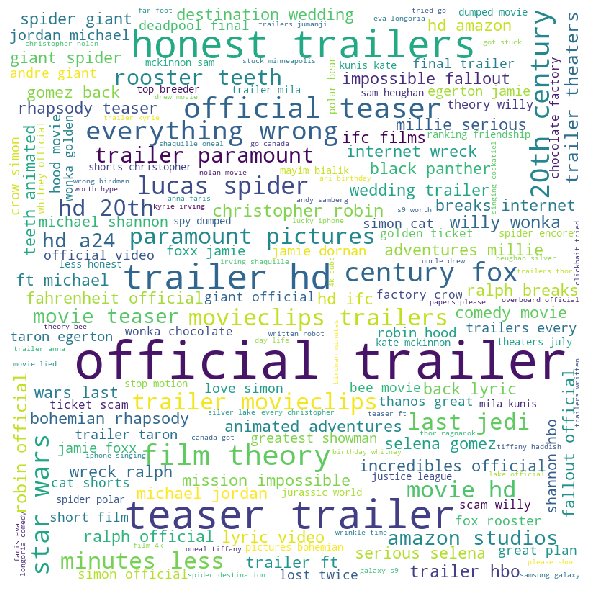
\includegraphics[width=\linewidth]{project/wc_1.png}
      \caption{Film \& Animation}\label{fig:awesome_image1}
    \endminipage\hfill
    \minipage{0.32\textwidth}
      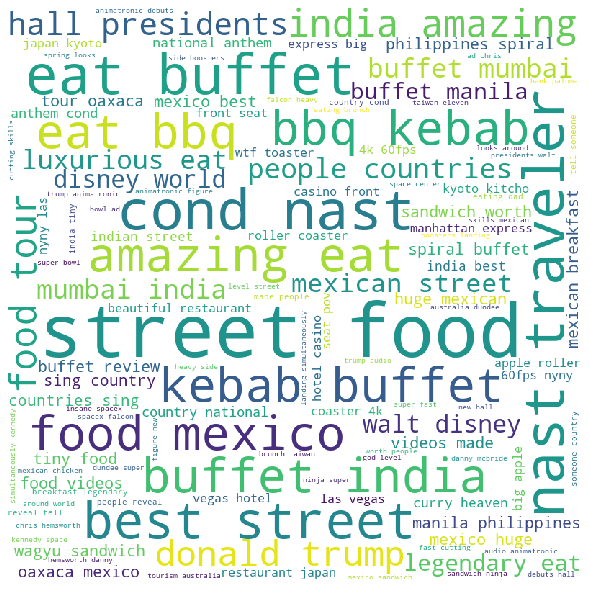
\includegraphics[width=\linewidth]{project/wc_19.png}
      \caption{Travel \& Events}\label{fig:awesome_image2}
    \endminipage\hfill
    \minipage{0.32\textwidth}%
      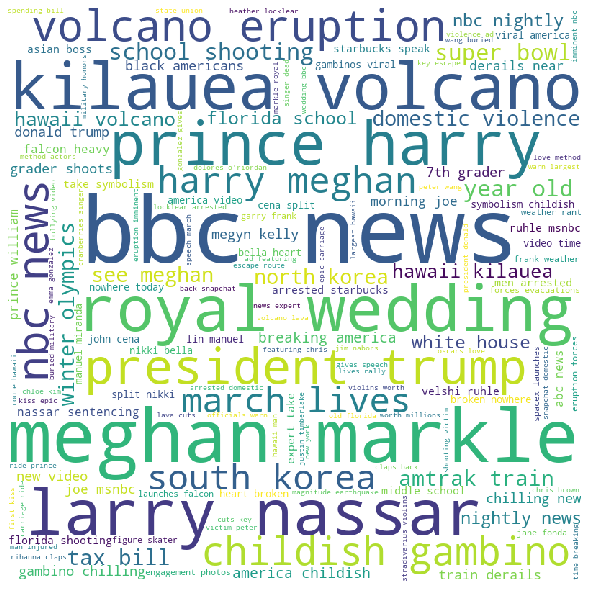
\includegraphics[width=\linewidth]{project/wc_25.png}
      \caption{News \& Politics} \label{fig:awesome_image3}
    \endminipage
    \end{figure}

    \end{enumerate}
    
    \subsection{Feature extraction}
    \begin{enumerate}
    \item Generate a word bank through removing top 10\% most frequent cleaned tags for each category in the data to avoid over-weighting the word bank. The format of the word bank: 
    \{category\_id: list of cleaned tags\}
    \item Use tokens generated 5.1.(e) step in description to generate potential category(ies) based on its frequency in the word bank.
    \item Use CountVectorizer to convert a text documents to a matrix of token counts.
    \item Use TF-IDF to train and transform training data.
    \end{enumerate}

\end{enumerate}

\section{Experiments and Results}
\subsection{Experiment 1}
\subsubsection{Experiment}
\begin{enumerate}
\item Instead of predicting specific view counts, this problem can be converted into classifying videos into view count buckets, where each bucket contains a view count range (e.g. 1 million to 2 million views). We split the view count, based on the min/max range of all the view counts, into 10 uniform buckets, while keeping interval size of each bucket the same. 
\item Convert ``views" for each sample in the dataset into a one-hot categorical label, corresponding to a bucket/class.
\item Construct and transformed raw text data into TF-IDF training/testing data, one feature at a time For this experiment, we used ``tag", ``description and ``title". 
\item Train a naive bayes model on transformed TF-IDF data and the labels generated from step (b).
\item Run the classifier to classify the test data into specific view buckets
\end{enumerate}
\subsubsection{Results}
\begin{enumerate}
    \item The results show that the most of classifications were concentrated in the first bucket, which led to further investigation of our bucket design and our second experiment.
    \item The investigation show that our input data had a right-skewed distribution for the ``views" feature, which led to the first two buckets to cover 90\% of all the samples.
    \begin{figure}[H]
        \centering
        \resizebox{4.5in}{!}{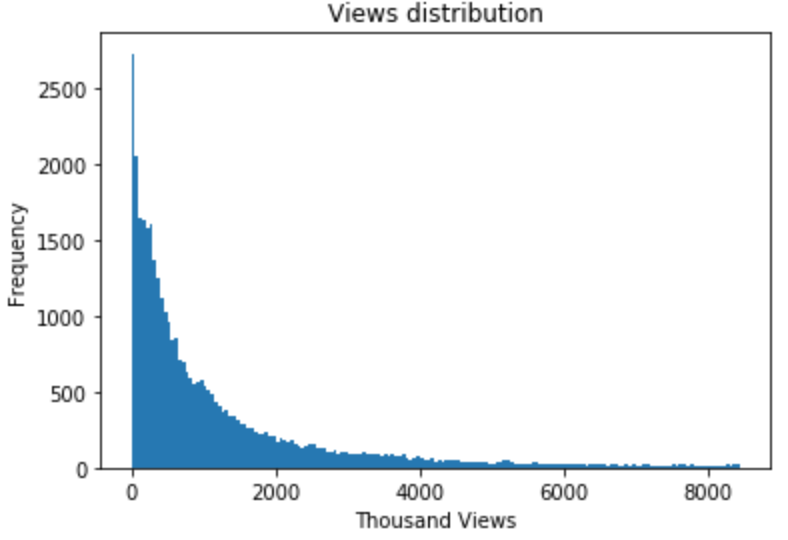
\includegraphics{project/view_distribution.png}}
        
        \caption{Views Distribution}
        \label{fig:my_label}
    \end{figure}
    
\end{enumerate}
\pagebreak
\subsection{Experiment 2}
\subsubsection{Experiment}
\begin{enumerate}
\item Split the raw view count, based on view count percentiles, into 10 uniform buckets, which keeps number of samples in each bucket the same. 
\item Convert ``views" for each sample in the dataset into a one-hot categorical label, corresponding to a bucket/class.
\item Train the same Naive Bayes classifier (in experiment 1), to verify that the bucket design alleviates the problem of having a skewed data distribution. For this experiment, we also only used ``tag", ``description" and ``title", one feature at a time.
\item Train the data on various of classifiers such as the random forest classifier, ridge regression classifier, stochastic gradient descent classifier, boosted gradient trees, and linear-SVM (one-vs-rest and one-vs-one scheme).
\item Run the classifier to classify test data into specific view buckets. We used ``title",``tags", and ``description" respectively to predict the view buckets on the test data.
\end{enumerate}

\subsubsection{Results}
\begin{enumerate}
\item The resulting redesign of the view buckets has a distribution of a uniform across all buckets (rectangular shape).
% 贴图
\item{Classification Accuracy Comparison}
\begin{table}[H]
\centering
\begin{tabular}{ *2c } 
 \toprule
 \textbf{Method} & \textbf{Accuracy (\%)}\\
 \midrule
 \multicolumn{2}{c}{\textit{Tags}} \\
 \midrule
 Ridge & 50.6 \\
 Linear SVM (one-vs-rest) & 49.2 \\
 Naive Bayes & 47.2 \\
 SGD & 44.5 \\
 Random Forest & 29.5 \\
 Gradient Tree Boosting & 26.5 \\
 Linear SVM (one-vs-one) & 14.1 \\
 \midrule
 \multicolumn{2}{c}{\textit{Description}} \\
 \midrule
 Naive Bayes & 33.0 \\
 Ridge & 27.9 \\
 SGD & 26.6 \\
 Linear SVM (one-vs-rest) & 26.3 \\
 Gradient Tree Boosting & 16.6 \\
 Random Forest & 13.5 \\
 Linear SVM (one-vs-one) & 12.2 \\
 \midrule
 \multicolumn{2}{c}{\textit{Title}} \\
 \midrule
 Naive Bayes & 21.8 \\
 Ridge & 20.8 \\
 Linear SVM (one-vs-rest) & 20.2 \\
 SGD & 20.2 \\
 Linear SVM (one-vs-one) & 17.2 \\
 Gradient Tree Boosting & 13.9 \\
 Random Forest & 13.6 \\
 \bottomrule
\end{tabular}
\label{nnOA}
\end{table}

\end{enumerate}


%\section{Conclusion and Discussion}

%\section*{Acknowledgments}

\newpage
%============================= BIBLIOGRAPHY ===============================

\bibliographystyle{plain}
\bibliography{references}

\end{document}